\documentclass[journal]{IEEEtran}

\usepackage{amsmath,amssymb,amsfonts}
\usepackage{algorithmic}
\usepackage{graphicx}
\usepackage{textcomp}
\usepackage{xcolor}
\usepackage{booktabs}
\usepackage{cite}
\usepackage{microtype}
\usepackage{url}
\usepackage{bm}
\usepackage{balance}

\setlength{\textfloatsep}{4pt plus 1pt minus 1pt}
\setlength{\floatsep}{3pt plus 1pt minus 1pt}
\setlength{\dbltextfloatsep}{4pt plus 1pt minus 1pt}
\setlength{\dblfloatsep}{3pt plus 1pt minus 1pt}
\setlength{\abovecaptionskip}{2pt plus 0.5pt minus 0.5pt}
\setlength{\belowcaptionskip}{1.5pt plus 0.5pt minus 0.5pt}
\setlength{\abovedisplayskip}{3pt plus 1pt minus 1pt}
\setlength{\belowdisplayskip}{3pt plus 1pt minus 1pt}
\setlength{\abovedisplayshortskip}{1pt plus 1pt minus 1pt}
\setlength{\belowdisplayshortskip}{1pt plus 1pt minus 1pt}


\begin{document}
\bstctlcite{IEEEexample:BSTcontrol}

\title{A Bedside Decision Support System for Disorders of Consciousness: Multi-Scale Temporal Dynamics and Multicenter Validation}

\author{Hongjie~Chen$^{1}$, Jianming~Chen$^{1}$, Guanyu~Xiong$^{2}$, Fang~Li$^{2}$, and Fang~Duan$^{1,*}$%
\thanks{$^{1}$Hongjie Chen, Jianming Chen, and Fang Duan are with the College of Information Science and Engineering, Huaqiao University, Xiamen 361021, China (e-mail: chenhj976@gmail.com; nkfetsh@gmail.com).}%
\thanks{$^{2}$Guanyu Xiong and Fang Li are with the China Rehabilitation Research Center, Beijing Bo'ai Hospital, Capital Medical University, Beijing, China.}%
\thanks{$^{*}$Corresponding author: Fang Duan (e-mail: nkfetsh@gmail.com).}%
}

\markboth{IEEE JOURNAL OF BIOMEDICAL AND HEALTH INFORMATICS}%
{Chen et al.: Bedside Decision Support System for Disorders of Consciousness}

\maketitle

\begin{abstract}
Bedside EEG summaries often discard temporal order, limiting assessment of residual consciousness in small clinical cohorts. We developed an interpretable framework combining physically adjacent lag-1 persistence ($\rho_1$), normalized jump rate ($D_1$), and common-mode-adjusted bilateral correlation ($r_{\text{residual}}$) with fixed-weight consensus scoring. Evaluation comprised two continuous EEG cohorts, one exploratory short-record dataset, and one sleep cohort ($N=129$ records). On long-term discovery EEG ($N=41$), the primary four-feature suite achieved 0.9324 AUROC under 25 subject-level outer partitions, compared with 0.8964 for the strongest supervised baseline using identical features and preprocessing (paired gain $+0.0360$, 95\% interval $[+0.0090,+0.0728]$). Sequence dependence of the lag-1 extension was verified by 10,000 synchronous shuffles, reducing its AUROC from 0.8911 to $0.8182\pm0.0049$ while preserving channel marginals and instantaneous spatial covariance. On China Rehabilitation Research Center telemetry ($N=15$), shared unlabeled target standardization and direction alignment yielded 0.7778 AUROC; fixed soft truncation ($c=1.5$) increased this to 0.7963, with matched supervised baselines at 0.7407--0.7593. On 120-s Figshare records ($N=50$), the jump-rate branch achieved 0.7691 AUROC, comparable to matched baselines at 0.7674--0.7759. Sleep-stage transition flexibility in the Wielek cohort ($N=23$) provided complementary evidence across circadian timescales. With 2.15~ms per evaluated update in cached-power replay, the framework provides a compact, auditable basis for bedside assessment and prioritization of further multimodal evaluation.
\end{abstract}

\begin{IEEEkeywords}
Disorders of consciousness (DoC), electroencephalography (EEG), temporal dynamics, clinical decision support systems (CDSS), mesocircuit hypothesis, consensus fusion.
\end{IEEEkeywords}

\section{Introduction}
\IEEEPARstart{S}{evere} acute brain injury from trauma, anoxia, or stroke leaves patients in prolonged disorders of consciousness (DoC), clinically categorized into the vegetative state/unresponsive wakefulness syndrome (VS/UWS) and the minimally conscious state (MCS)~\cite{giacino2002minimally,giacino2018practice}. Distinguishing MCS from VS/UWS informs decisions on withdrawing life-sustaining treatment, administering analgesia, and projecting rehabilitation potential. Bedside clinical evaluations carry an estimated 40\% misdiagnosis rate~\cite{schnakers2009diagnostic}. Although standardized assessments such as the Coma Recovery Scale-Revised (CRS-R)~\cite{schnakers2009diagnostic} reduce diagnostic error, motor impairment and fluctuating arousal frequently confound behavioral examinations~\cite{cruse2011bedside}. Furthermore, prospective cohorts establish that 15\%--35\% of behaviorally unresponsive patients exhibit cognitive-motor dissociation (CMD)~\cite{bodien2024cognitive}, retaining volitional cortical responses despite absent motor output.

Functional neuroimaging and perturbational protocols (fMRI, $^{18}\text{F}$-FDG PET, TMS-EEG)~\cite{casali2013theoretically,chennu2017brain} show that preserved cortical complexity differentiates MCS from VS/UWS, but the hazards of intra-hospital transport preclude routine bedside deployment in the intensive care unit. Sparse continuous EEG (4--8 electrodes) provides the primary practical modality for longitudinal monitoring~\cite{sitt2014large,engemann2018robust,bareham2020spectral}. Beyond static power spectra, prior investigations examined non-linear entropy~\cite{bandt2002permutation,sitt2014large}, microstates~\cite{ling2024microstates}, sleep architecture~\cite{wielek2018sleep,xiao2026sleep}, long-range temporal correlations via detrended fluctuation analysis (DFA)~\cite{thiery2018long,wei2023aberrant}, source-space connectivity~\cite{bai2021spontaneous}, and dynamical criticality~\cite{toker2022consciousness}. However, clinical bedside translation remains constrained: multi-scale DFA requires stationary dense montages; source reconstruction is ill-posed with sparse arrays; entropy measures exhibit marked artifact sensitivity; and flexible classifiers risk overfitting under small discovery cohorts ($N_{\text{train}} \approx 32$). Bedside assessment has therefore relied on empirical band power, marginal dispersion ($-\mathrm{CV}_\theta$), and unadjusted bilateral correlations~\cite{bareham2020spectral,wielek2018sleep}. As a result, non-invasive bedside discrimination has remained bounded to a moderate plateau (0.75--0.82 AUROC).

\subsection{The Permutation Invariance Defect of Conventional Metrics}
This diagnostic plateau stems from a shared limitation: strict permutation invariance. Conventional pipelines rely on aggregate dispersion ($-\mathrm{CV}_\theta$) and instantaneous bilateral correlation ($r_{\text{interhem}}$), which are mathematically invariant ($\approx 10^{-15}$ under index shuffling). Treating continuous EEG trajectories as unordered sets discards directional multi-second continuity and cortical reverberation.

\subsection{The Mesocircuit Hypothesis and Autoregressive Memory}
This methodological gap diverges from established neurobiology of conscious recovery, specifically the anterior forebrain mesocircuit hypothesis~\cite{schiff2010recovery}. Under this framework, sustained behavioral awareness depends on recurrent reciprocal excitatory loops linking the central thalamus, striatum, and frontoparietal association cortices. Preserved mesocircuit connectivity manifests electrophysiologically as multi-second autoregressive continuity, quantifiable via lag-1 autocorrelation ($\rho_1$) across consecutive epochs. In VS/UWS, widespread structural deafferentation and loss of striatal inhibition disinhibit the internal globus pallidus (GPi), which drives sustained hyperpolarization of the central thalamus and degrades cortical activity into memoryless fluctuations. Differentiating conscious capacity from reflexive unresponsiveness therefore requires operators sensitive to physical sequence persistence.

As illustrated in Fig.~\ref{fig:schematic}a, individual theta trajectories in MCS (e.g., patient P36) exhibit sustained multi-second wave-holding, whereas VS/UWS trajectories (e.g., patient P25) break into decoupled transients. Static dispersion ($-\mathrm{CV}_\theta$) displays substantial individual overlap between cohorts ($p = 0.0264$; Fig.~\ref{fig:schematic}c), whereas lag-1 persistence ($\rho_1$) reliably separates conscious from unresponsive states ($p = 0.0227$; Fig.~\ref{fig:schematic}b). 

While continuous multi-hour telemetry enables stable asymptotic estimation of $\rho_1$, emergency bedside triage frequently relies on ultra-short recordings ($< 5$~min). In this small-sample regime, sample autocorrelation exhibits elevated estimator variance ($\operatorname{Var}(\hat{\rho}_1) \sim \mathcal{O}(1/M)$). For brief recordings, we introduce the normalized jump rate ($D_1$) across verified adjacent epochs ($\mathbb{I}_{\text{adj}} = 1$), which analytically unifies static amplitude dispersion and temporal decay via $D_1 \approx 2\pi^{-1/2}(-\mathrm{CV}_\theta)(1-\rho_1)^{1/2}$.

\begin{figure*}[t]
\centering
\vspace{-4pt}
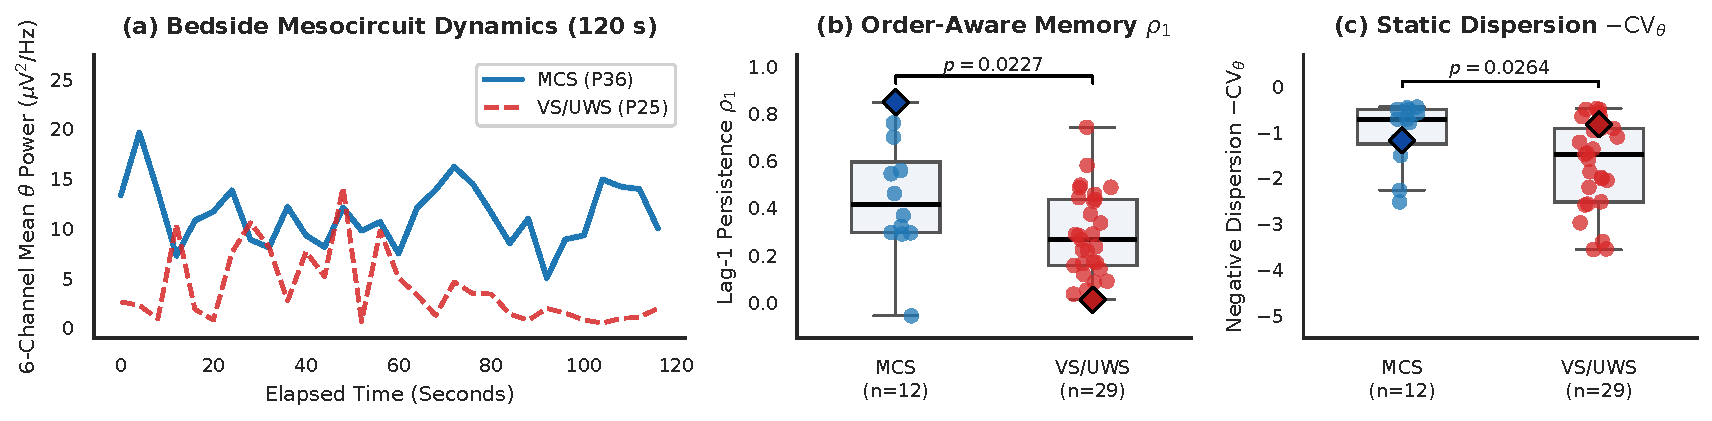
\includegraphics[width=0.80\textwidth]{figures/fig1_mesocircuit_memory.pdf}
\vspace{-3pt}
\caption{Bedside EEG dynamics and patient distributions. (a) Standardized theta power across 30 consecutive 4-s epochs in P36 (MCS) and P25 (VS/UWS). (b,c) Lag-1 persistence $\rho_1$ ($p=0.0227$) and positive theta CV ($p=0.0264$) across 12 MCS and 29 VS/UWS patients (two-sided Mann--Whitney tests). Jittered points show all individual patients; boxes show medians and IQRs; whiskers span 1.5 IQR. Panel c uses a logarithmic scale for theta CV.}
\label{fig:schematic}
\vspace{-3pt}
\end{figure*}

\subsection{Spurious Bilateral Coupling Driven by Diffuse Slow Waves}
Diffuse slow-wave volume conduction also confounds bilateral bedside monitoring. In acute brain injury, high-amplitude delta and theta oscillations propagate broadly across the scalp via volume conduction and subcortical pacemaking. Although common average reference (CAR) subtracts linear potential offsets, rectified band-power envelopes retain substantial shared variance ($R^2 \approx 47\%$) from global pacemaking. This shared background inflates raw inter-hemispheric correlation and obscures regional differentiation. Decoupling this common mode via ordinary least squares (OLS) orthogonal projection isolates residual bilateral resonance ($r_{\text{residual}}$), separating pathological co-activation in VS/UWS from preserved modular dynamics in MCS.

\subsection{Contributions of This Work}
This study introduces an interpretable bedside decision support framework with three principal contributions:

1) \textit{Order-aware temporal operators and artifact decoupling}: We formulate lag-1 autocorrelation ($\rho_1$) for continuous telemetry alongside normalized adjacent jump rates ($D_1$) for short recordings under physical adjacency constraints ($\mathbb{I}_{\text{adj}} = 1$), analytically unified via $D_1 \approx 2\pi^{-1/2}(-\mathrm{CV}_\theta)(1-\rho_1)^{1/2}$. Synchronously shuffling 10,000 surrogate sequences reduces classification performance from 0.8911 AUROC to permutation baseline ($0.8182 \pm 0.0049$, $p < 0.0001$), confirming that diagnostic separation depends on physical sequence order rather than static marginal distributions. Ordinary least squares (OLS) orthogonal projection decouples shared slow-wave envelope variance ($R^2 \approx 47\%$) to isolate genuine bilateral resonance ($r_{\text{residual}}$).

2) \textit{Interpretable, parameter-free bedside consensus}: The parsimonious four-feature suite $\mathbf{x}_{\text{ortho}}=[c_{\text{global}},-\mathrm{CV}_\theta,\rho_1,r_{\text{residual}}]^\top$ attains 0.9324 AUROC and 0.8998 average precision (AP) on primary discovery telemetry. Given identical feature inputs, equal-weight consensus scoring exceeds the top-performing matched supervised model (logistic regression) by $+0.0360$ AUROC (Dirichlet paired 95\% confidence interval $[+0.0090, +0.0728]$), requiring 2.15~ms per evaluated update in cached-power replay (Supplementary Note~D).

3) \textit{Multicenter evaluation across distinct acquisition settings}: The framework is validated across 129 records spanning four independent cohorts: CRRC telemetry ($N=15$) establishes cross-hardware generalization (0.7778 to 0.7963 AUROC); Figshare 120-second recordings ($N=50$) demonstrate emergency triage utility (0.7691 AUROC); and Wielek polysomnography ($N=23$) confirms preservation of macro-scale sleep stage transitions across circadian cycles.

\section{Mathematical Formulation and Methods}

Fig.~\ref{fig:system_workflow} summarizes the processing, scoring and evaluation workflow.
\begin{figure*}[t]
\centering
\vspace{-4pt}
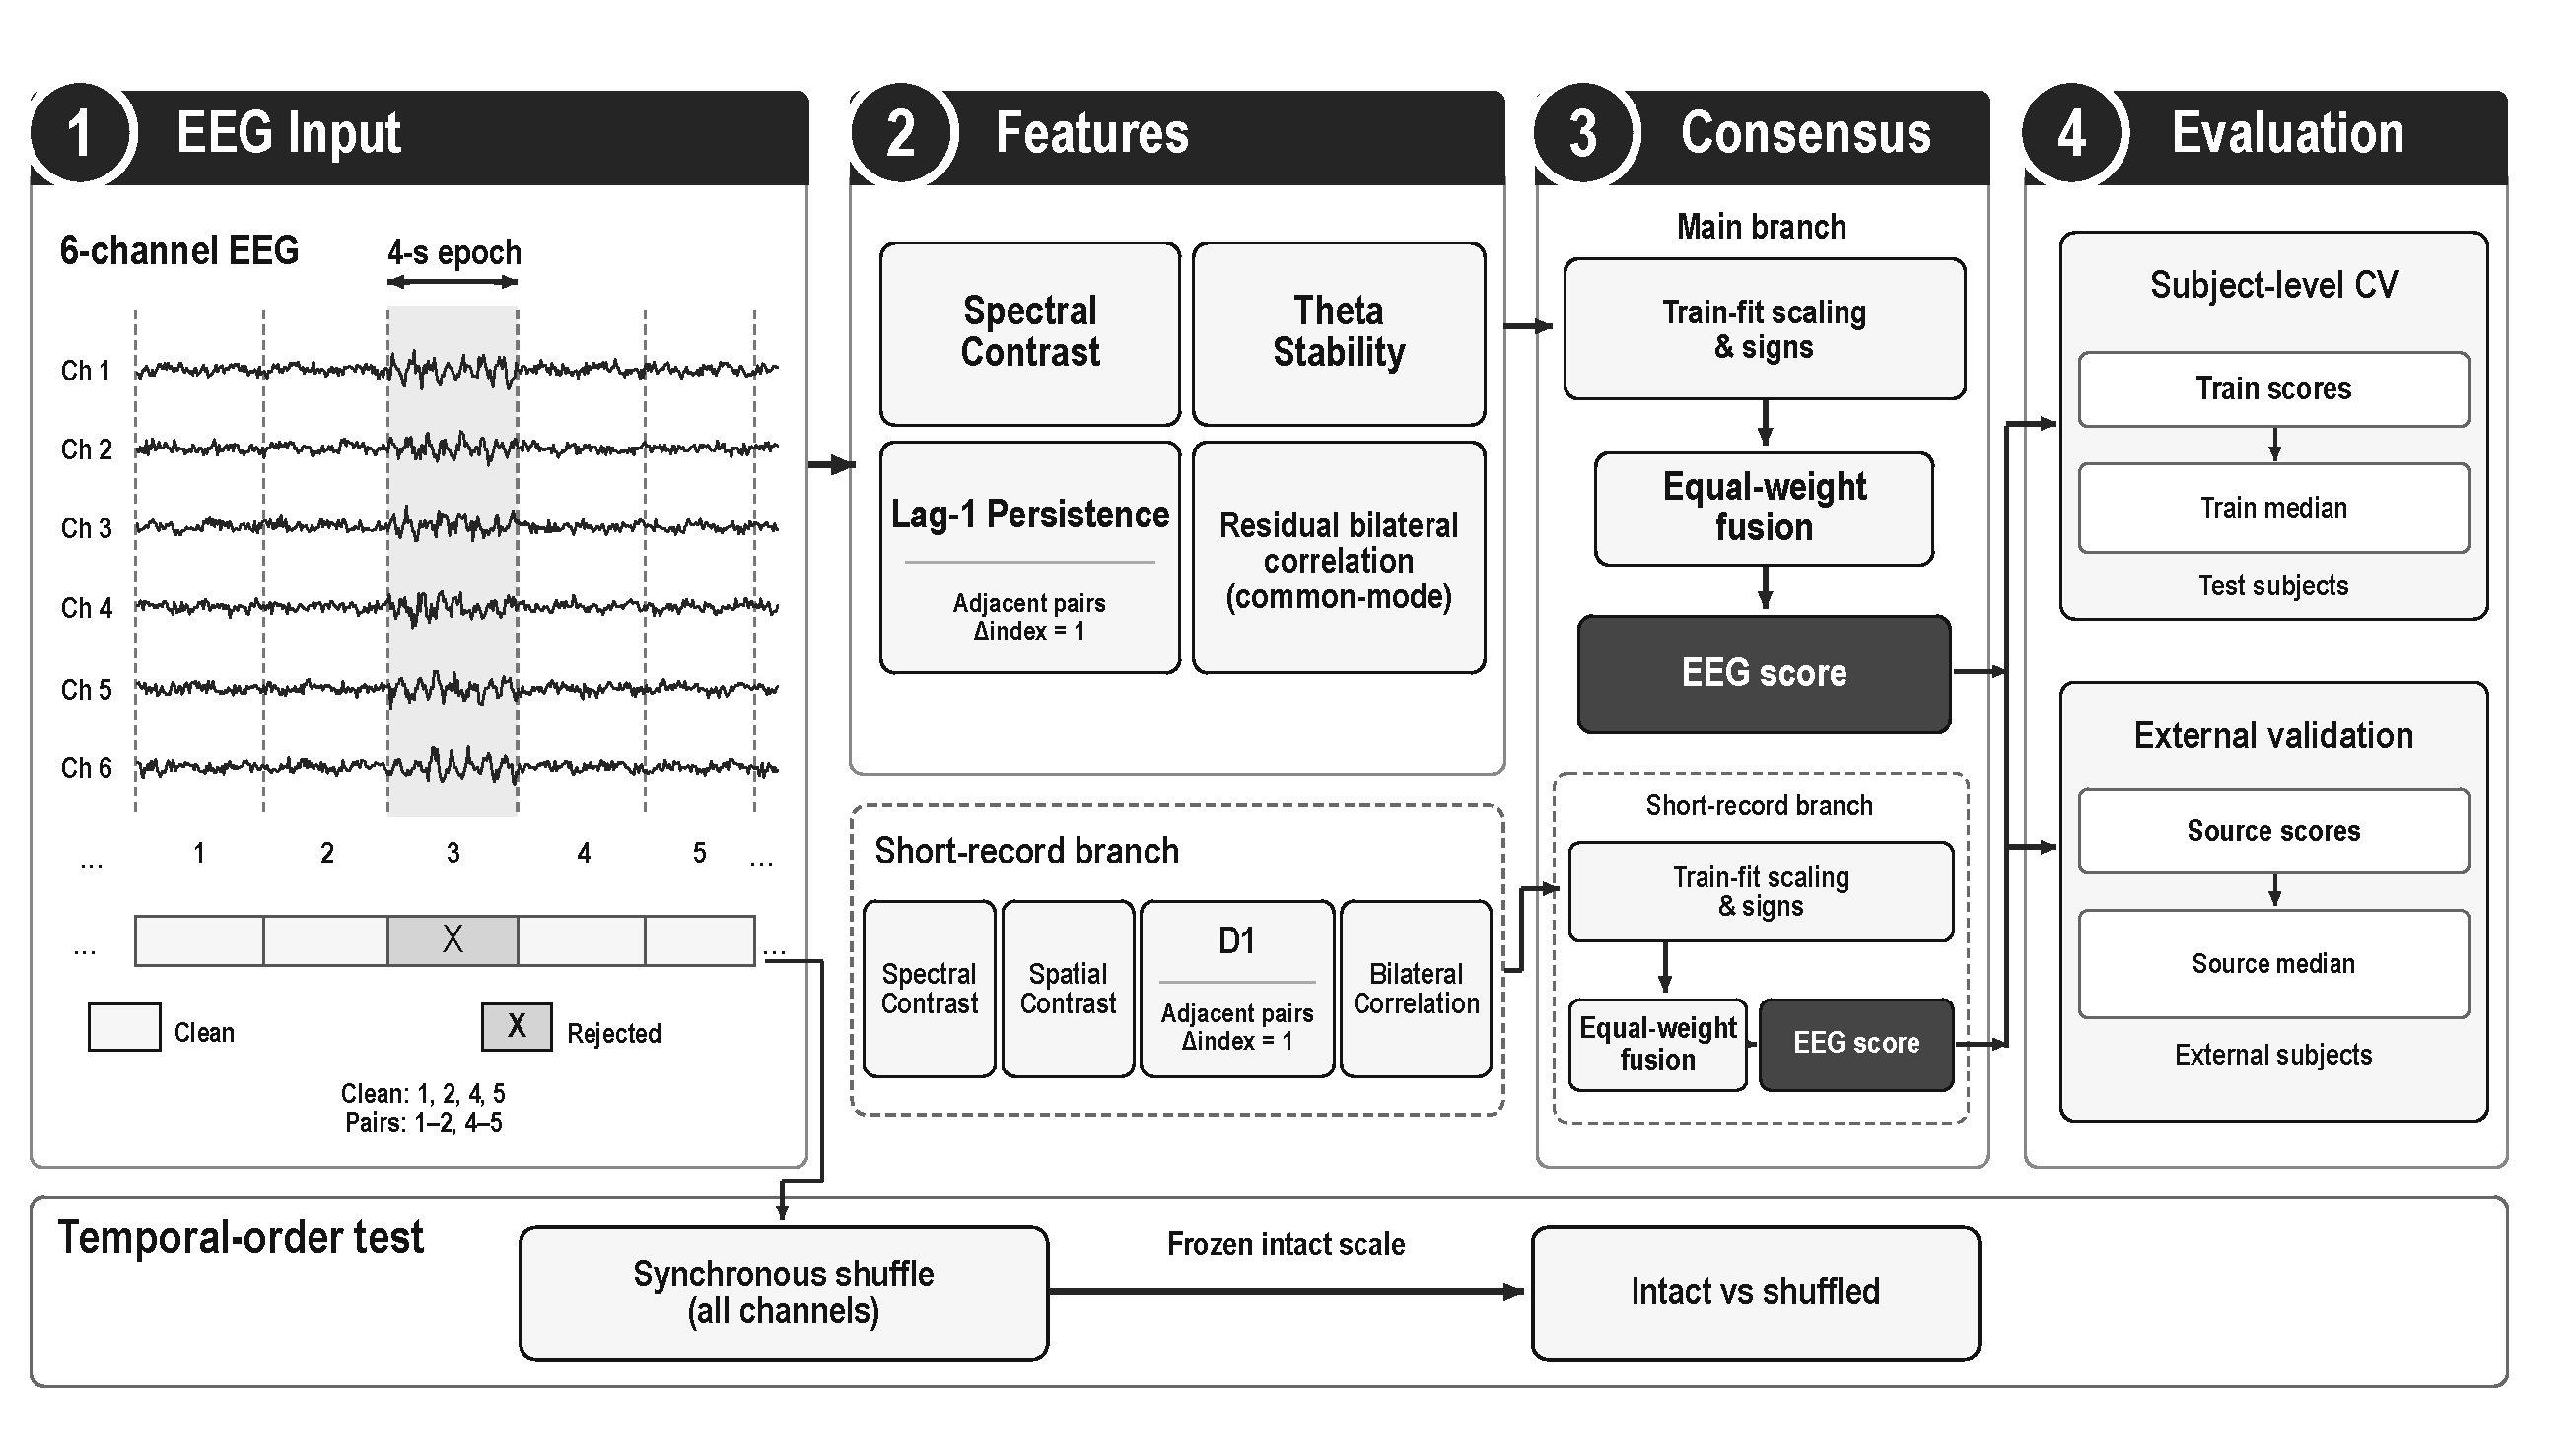
\includegraphics[width=0.76\textwidth]{figures/fig_system_workflow.pdf}
\vspace{-3pt}
\caption{System overview. Schematic EEG traces illustrate processing. Original block indices are preserved for physical adjacency. Main and short-record branches use distinct 4-feature suites with parameter-free equal-weight consensus scoring. Discovery uses 4-s epochs; Figshare triage uses 2-s segments. Source training folds fix scaling, signs, and operating medians. External cohorts include target-batch standardization and direction alignment where indicated. Shuffled surrogate tests use 10,000 synchronous permutations with frozen scales.}
\label{fig:system_workflow}
\vspace{-4pt}
\end{figure*}

\subsection{Clinical Cohorts and Ethical Compliance}
Four multicenter cohorts totaling $N=129$ records were evaluated under institutional ethical approvals:

\textbf{1) Mendeley Discovery Cohort} ($N = 41$): Continuous 6-channel bedside EEG (F3, F4, C3, C4, O1, O2; 256~Hz) from 41 patients with severe brain injuries at FRCCICMR Moscow~\cite{nekrasova2020psg}: 12 MCS (8 $\text{MCS}^+$, 4 $\text{MCS}^-$; duration $6.00 \pm 0.00$~h) and 29 VS/UWS ($5.97 \pm 0.61$~h), diagnosed through repeated CRS-R assessments.

\textbf{2) CRRC Inpatient Cohort} ($N = 15$): Prospective bedside telemetry from 15 subacute male patients (6 MCS, 9 VS/UWS; 11 ICH, 4 TBI; age $51.7 \pm 12.3$~years, range $28\text{--}69$; duration $19.5 \pm 8.0$~min; Ethics No.~2025-118-01~\cite{duan2026auditory}) at China Rehabilitation Research Center (CRRC). Data were acquired with a 32-channel NeuSen NSM2 system (1000~Hz, 4-second blocks) during stable post-acute rehabilitation (Supplementary Note~A). Homologous 6 channels were evaluated; mechanical drift at $O_2$ in two patients (CRRC\_008, CRRC\_009) yielded a pristine subgroup of $N = 13$ (6 MCS including 1 EMCS, 7 VS/UWS).

\textbf{3) Figshare Short-Record Analysis} ($N = 50$): High-density resting-state EEG (250~Hz, 120-s) from 50 patients with prolonged DoC (19 MCS, 31 VS/UWS) at Hangzhou Mingzhou Brain Rehabilitation Hospital~\cite{ling2024microstates,xu2021neural}, evaluating frozen-source scoring on homologous channels. Published group counts support the 19 MCS and 31 VS/UWS composition; file-level diagnosis mapping and intersegment continuity require independent confirmation.

\textbf{4) Wielek PSG Cohort} ($N = 23$): 24-hour polysomnography from 23 post-comatose patients (11 MCS, 12 VS/UWS)~\cite{wielek2018sleep}, with 30-second hypnograms (Wake, N1, N2, N3, REM) tracking macro-scale transition continuity across circadian sleep cycles.
\subsection{EEG Acquisition, Preprocessing, and Physical Adjacency Constraint}
\begin{table*}[t]
\centering
\renewcommand{\arraystretch}{0.88}
\footnotesize
\caption{Performance of Order-Aware Temporal Dynamics, Consensus Fusion, and Machine Learning Baselines on Mendeley Cohort (25 Outer Partitions; 95\% CIs paired vs. Canonical Linear Baseline via 10,000 Dirichlet resamples; PR-AUC reported as Average Precision [AP], with trapezoidal PR-AUC = 0.8782 for 4-Feat Linear; matched supervised rows use the same four features as the deployment suite; 5-Feat combined models substitute $r_{\text{interhem}}$ with $r_{\text{res}}$).}
\label{tab:main_results}
\begin{tabular}{lcccccc}
\hline
\textbf{Model / Feature Configuration} & \textbf{AUROC} & \textbf{PR-AUC} & \textbf{Balanced Acc.} & \textbf{Sensitivity} & \textbf{Specificity} & \textbf{95\% CI vs. Baseline} \\
\hline
\multicolumn{7}{l}{\textit{Consensus Aggregation Frameworks}} \\
\hline
\quad Canonical Static (4 Feats, Linear) & 0.8200 & 0.7823 & 0.7201 & 0.8333 & 0.6069 & Baseline \\
\quad Canonical Static (4 Feats, Rank Consensus) & 0.7893 & 0.7299 & 0.7270 & 0.8333 & 0.6207 & {$[-0.0619, -0.0076]$} \\
\quad Plus Lag-1 $\rho_1$ (5 Feats, Linear) & \textbf{0.8911} & \textbf{0.8384} & \textbf{0.7997} & 0.9167 & 0.6828 & {$[+0.0011, +0.1534]$} \\
\quad Plus Lag-1 $\rho_1$ (5 Feats, Rank Consensus) & 0.8591 & 0.8068 & 0.7187 & 0.8167 & 0.6207 & {$[-0.0188, +0.1053]$} \\
\quad Plus $\rho_1 + r_{\text{res}}$ (5 Feats, Linear, $c=1.5\sigma$) & \textbf{0.9149} & \textbf{0.8782} & \textbf{0.8399} & 0.9833 & 0.6966 & {$[+0.0064, +0.1931]$} \\
\quad Plus $\rho_1 + r_{\text{res}}$ (5 Feats, Rank Consensus) & 0.8949 & 0.8353 & 0.7741 & 0.9000 & 0.6483 & {$[+0.0049, +0.1530]$} \\
\quad T-GECF Adaptive Gated Hybrid (5 Feats) & \textbf{0.9116} & \textbf{0.8669} & \textbf{0.8399} & 0.9833 & 0.6966 & {$[+0.0013, +0.1927]$} \\
\hline
\multicolumn{7}{l}{\textit{Supervised \& Domain Baseline Benchmarks}} \\
\hline
\quad Lempel-Ziv Complexity (LZC) & 0.5136 & 0.5061 & 0.4973 & 0.5133 & 0.4813 & {$[-0.4229, -0.1861]$} \\
\quad Shannon Spectral Entropy (SE) & 0.6953 & 0.6182 & 0.6967 & 0.7933 & 0.6000 & {$[-0.2508, +0.0073]$} \\
\quad Canonical Static (Tuned Ridge) & 0.7653 & 0.7193 & 0.6661 & 0.7667 & 0.5655 & {$[-0.0998, -0.0140]$} \\
\quad Orthogonal 4-Feat (Tuned Ridge) & 0.8813 & 0.8393 & 0.7825 & 0.9167 & 0.6483 & {$[-0.0446, +0.1744]$} \\
\quad Canonical Static (Tuned Logistic) & 0.7722 & 0.7236 & 0.6917 & 0.7833 & 0.6000 & {$[-0.0959, -0.0064]$} \\
\quad Orthogonal 4-Feat (Tuned Logistic) & 0.8964 & 0.8524 & 0.8080 & 0.9333 & 0.6828 & {$[-0.0225, +0.1826]$} \\
\quad Canonical Static (Shrinkage-LDA) & 0.7709 & 0.7252 & 0.6626 & 0.7667 & 0.5586 & {$[-0.0884, -0.0162]$} \\
\quad Orthogonal 4-Feat (Shrinkage-LDA) & 0.8769 & 0.8424 & 0.7859 & 0.9167 & 0.6552 & {$[-0.0496, +0.1699]$} \\
\hline
\multicolumn{7}{l}{\textit{Representation Ablations \& Operator Variants}} \\
\hline
\quad Plus Jump $D_1$ (5 Feats, Linear) & 0.8611 & 0.8012 & 0.7491 & 0.8500 & 0.6483 & {$[-0.0018, +0.0911]$} \\
\quad Plus Jump $D_1$ (5 Feats, Rank Consensus) & 0.8424 & 0.7787 & 0.7132 & 0.8333 & 0.5931 & {$[-0.0208, +0.0694]$} \\
\quad Replace $-\mathrm{CV}_\theta$ with $\rho_1$ (Linear) & 0.8851 & 0.8495 & 0.7678 & 0.8667 & 0.6690 & {$[-0.0223, +0.1613]$} \\
\quad Replace $-\mathrm{CV}_\theta$ with $D_1$ (Linear) & 0.8720 & 0.8097 & 0.7776 & 0.9000 & 0.6552 & {$[+0.0050, +0.1094]$} \\
\quad Residual Correlation $r_{\text{res}}$ (Linear) & 0.8433 & 0.7671 & 0.7575 & 0.8667 & 0.6483 & {$[-0.0561, +0.1070]$} \\
\quad Orthogonal 4-Feat (Drop $c_{\text{spatial}}$, Linear) & \textbf{0.9324} & \textbf{0.8998} & \textbf{0.8101} & 0.9167 & 0.7034 & {$[+0.0174, +0.2186]$} \\
\quad Orthogonal 4-Feat (Drop $c_{\text{spatial}}$, Rank Consensus) & \textbf{0.9076} & \textbf{0.8548} & \textbf{0.8448} & 1.0000 & 0.6897 & {$[+0.0137, +0.1725]$} \\
\hline
\end{tabular}
\end{table*}

\label{sec:preprocessing}
Continuous 6-channel EEG (256~Hz) was re-referenced to Common Average Reference (CAR) and segmented into non-overlapping 4-second epochs (1,024 samples). Spectral densities were computed across each epoch via Hann-tapered periodograms ($\Delta f = 0.25$~Hz), extracting theta (4--8~Hz) and alpha (8--13~Hz) band power.

Artifact screening at $500\,\mu\mathrm{V}$ retained $5{,}185.5 \pm 595.6$ blocks per patient ($96.98\% \pm 3.2\%$, $5.76 \pm 0.66$~h; rejection $2.84\% \pm 2.1\%$ in MCS vs. $3.09\% \pm 3.6\%$ in VS/UWS, $p=0.82$, Mann--Whitney $U$ test). A conservative $150\,\mu\mathrm{V}$ cutoff retained $90.14\% \pm 17.87\%$ blocks ($4{,}672.9 \pm 1{,}024.7$ pairs; minimum 668), confirming balanced retention across groups.

Let $\mathcal{T} = \{t_1, t_2, \dots, t_N\}$ denote clean epoch indices in a continuous session, and let $G_{t_i}$ denote spatial mean theta power across all 6 channels at epoch $t_i$. To prevent spurious concatenation across artifact gaps, the physical adjacency indicator is defined as:
\begin{equation}
\mathbb{I}_{\text{adj}}(t_i, t_{i+1}) = 
\begin{cases}
1, & \text{if } t_{i+1} - t_i = 1, \\
0, & \text{otherwise},
\end{cases}
\end{equation}
where 0 denotes an intervening artifact gap, and $\mathbb{I}_{\text{adj}} = 1$ denotes consecutive epochs. Sequential metrics operate strictly on pairs with $\mathbb{I}_{\text{adj}} = 1$, retaining $M = 5{,}133.3 \pm 687.7$ adjacent pairs per patient (minimum 1,678, exceeding the validity threshold $M \ge 10$).

\subsection{Canonical Static Features and Order-Aware Dynamics}
Four baseline features define $\mathbf{x}_{\text{canonical}} = [c_{\text{global}}, \allowbreak c_{\text{spatial}}, \allowbreak -\mathrm{CV}_\theta, \allowbreak r_{\text{interhem}}]^\top \allowbreak \in \mathbb{R}^4$. We evaluate three expanded feature spaces: the 5-feature temporal extension $\mathbf{x}_{+\rho_1} = [c_{\text{global}}, c_{\text{spatial}}, -\mathrm{CV}_\theta, r_{\text{interhem}}, \rho_1]^\top \in \mathbb{R}^5$; the 5-feature combined suite $\mathbf{x}_{\text{combined}} = [c_{\text{global}}, c_{\text{spatial}}, -\mathrm{CV}_\theta, \rho_1, r_{\text{residual}}]^\top \in \mathbb{R}^5$; and the primary parsimonious 4-feature deployment suite $\mathbf{x}_{\text{ortho}} = [c_{\text{global}}, -\mathrm{CV}_\theta, \rho_1, r_{\text{residual}}]^\top \in \mathbb{R}^4$. Theta power (4--8~Hz) serves as the primary carrier because thalamocortical mesocircuit projections drive frontoparietal dynamics within this band~\cite{schiff2010recovery}, whereas delta reflects non-specific slowing and alpha is largely abolished in VS/UWS. Let $P_{\theta, t}^{(k)}$ and $P_{\alpha, t}^{(k)}$ denote theta and alpha powers of channel $k \in \{1, \dots, 6\}$ at clean epoch $t \in \{1, \dots, N\}$.

\textbf{1) Global Spectral Contrast ($c_{\text{global}}$)}: Quantifies the ratio of slow to fast power across all channels: $c_{\text{global}} = (\bar{P}_\theta - \bar{P}_\alpha)/(\bar{P}_\theta + \bar{P}_\alpha + \epsilon)$, where $\bar{P}_\theta = \frac{1}{6N}\sum_{k, t} P_{\theta, t}^{(k)}$, $\bar{P}_\alpha = \frac{1}{6N}\sum_{k, t} P_{\alpha, t}^{(k)}$, and $\epsilon = 10^{-12}$.

\textbf{2) Spatial Contrast ($c_{\text{spatial}}$)}: Computes mean slow-to-fast ratio: $c_{\text{spatial}} = \frac{1}{6}\sum_{k=1}^6 (\bar{P}_\theta^{(k)} - \bar{P}_\alpha^{(k)})/(\bar{P}_\theta^{(k)} + \bar{P}_\alpha^{(k)} + \epsilon)$. Fixed feature configurations were compared to assess spectral redundancy; the four-feature suite omitted spatial contrast (Section~III-C).

\textbf{3) Negative Theta Dispersion ($-\mathrm{CV}_\theta$)}: Measures temporal variance of mean theta $G_t = \frac{1}{6}\sum_{k=1}^6 P_{\theta, t}^{(k)}$: $-\mathrm{CV}_\theta = - \sqrt{\frac{1}{N}\sum_{t=1}^N (G_t - \bar{G})^2}/(\bar{G} + \epsilon)$, with temporal mean $\bar{G} = \frac{1}{N}\sum_{t=1}^N G_t$.

\textbf{4) Inter-Hemispheric Bilateral Correlation ($r_{\text{interhem}}$)}: Averages raw pairwise Pearson correlations across symmetric bilateral pairs: $r_{\text{interhem}} = \frac{1}{3}\sum_{(L, R)} \operatorname{Corr}(\mathbf{y}_L, \mathbf{y}_R)$, where $\mathbf{y}_L, \mathbf{y}_R \in \mathbb{R}^N$ denote the 4-second block theta-power vectors across symmetric pairs $(L, R) \in \{(\text{F3}, \text{F4}), (\text{C3}, \text{C4}), (\text{O1}, \text{O2})\}$.

To capture multi-second sequential continuity, two order-aware temporal representations are formulated on physically adjacent blocks:

\textbf{Lag-1 Memory Persistence ($\rho_1$)}: Quantifies autoregressive temporal persistence across consecutive 4-second blocks:
\begin{equation}
\rho_1 = \operatorname{Corr}(\{G_{t_i} \mid \mathbb{I}_{\text{adj}}=1\}, \{G_{t_{i+1}} \mid \mathbb{I}_{\text{adj}}=1\}).
\end{equation}
High $\rho_1$ values reflect smooth baseline preservation, whereas low values signify rapid temporal decorrelation.

\textbf{Normalized Adjacent Jump Rate ($D_1$)}: Measures resistance to high-frequency baseline discontinuities:
\begin{equation}
D_1 = - \frac{1}{M}\sum_{i: \mathbb{I}_{\text{adj}}=1} |G_{t_{i+1}} - G_{t_i}| / (\bar{G} + \epsilon),
\end{equation}
where $\bar{G} = \frac{1}{N}\sum_{t=1}^N G_t$, $M = \sum \mathbb{I}_{\text{adj}}$, and $\epsilon = 10^{-12}$. Under stationary Gaussian increments $\Delta G_t \sim \mathcal{N}(0, 2\sigma^2(1 - \rho_1))$, expected jump magnitude satisfies $\mathbb{E}[|\Delta G_t|] = 2\pi^{-1/2} \sigma (1 - \rho_1)^{1/2}$, yielding $D_1 \approx 2\pi^{-1/2} (-\mathrm{CV}_\theta) (1 - \rho_1)^{1/2}$. Evaluating $D_1$ on log-power increments accounts for 93.91\% of empirical variance under this identity (Section~\ref{sec:results_ablation}). Given estimator variance $\operatorname{Var}(\hat{\rho}_1) \sim \mathcal{O}(1/M)$, $D_1$ provides a low-variance proxy for brief records ($M < M^* \approx 75$ epochs), whereas $\rho_1$ achieves asymptotic efficiency.

To test macro-scale persistence on the Wielek PSG cohort ($N=23$), stage stay persistence on 30-s hypnograms $\{s_t\}_{t=1}^L \in \{\text{Wake, N1, N2, N3, REM}\}$ is $P_{\text{stay}} = \frac{1}{L-1}\sum_{t=1}^{L-1} \mathbb{I}(s_{t+1} = s_t)$, with transition flexibility $T_{\text{trans}} = 1 - P_{\text{stay}}$.
 
Together, these features form a hierarchical evaluation system. The four-dimensional feature space is spanned by four complementary physical domains: spectral slowing contrast, marginal envelope dispersion, sequential autoregressive continuity, and residual bilateral differentiation. The parsimonious 4-feature suite $[c_{\text{global}}, -\mathrm{CV}_\theta, \rho_1, r_{\text{residual}}]$ serves as the primary clinical deployment system, while orthogonal factorials and channel ablations systematically verify the independent contribution of each physical operator.

\subsection{Residual Bilateral Resonance ($r_{\text{residual}}$)}
\begin{table}[t]
\centering
\caption{Multiscale Sensitivity and External Cohort Benchmarks}
\label{tab:multiscale_sensitivity}
\vspace{-4pt}
\footnotesize
\renewcommand{\arraystretch}{0.84}
\setlength{\tabcolsep}{2.0pt}
\begin{tabular*}{\columnwidth}{@{\extracolsep{\fill}}lcc}
\hline
\multicolumn{3}{c}{\textbf{(A) Multiscale Window \& Cohort Transfer (AUROC)}} \\
\hline
\textbf{Cohort / Duration} & \textbf{Linear} & \textbf{Rank Consensus} \\
\hline
Mendeley 2-second & 0.8916 & 0.8529 \\
Mendeley 4-second (Default) & \textbf{0.8911} & \textbf{0.8591} \\
Mendeley 8-second & 0.8711 & 0.8453 \\
Mendeley 30-min Trunc. & 0.8867 & 0.8480 \\
Figshare Static Baseline & 0.7199 & 0.6812 \\
Figshare 120-s ($N=50$, Jump $D_1$) & \textbf{0.7691} & 0.6927 \\
Figshare 120-s ($N=50$, Lag-1 $\rho_1$) & 0.7012 & 0.6845 \\
Figshare 25-Fold CV ($D_1$, $N=50$) & \textbf{0.7771} & 0.7505 \\
\hline
\end{tabular*}
\vspace{2pt}
\noindent\begin{tabular*}{\columnwidth}{@{\extracolsep{\fill}}lc}
\hline
\multicolumn{2}{c}{\textbf{(B) Longitudinal \& Multi-Tier Benchmarks}} \\
\hline
\textbf{Validation Metric} & \textbf{Value} \\
\hline
Mendeley 5-h ICC ($\rho_1$ / $D_1$ / $r_{\text{residual}}$) & 0.4857 / 0.6433 / 0.4511 \\
Wielek Transition AUC (directional $p=0.030$) & \textbf{0.7348} \\
Wielek Mean State Stay (MCS vs. VS) & 0.7393 vs. 0.8361 \\
Figshare Zero-Shot BA (Train Thresh.) & 0.5645 (Sens 1.000) \\
62-Channel HD Mode-1 $R^2$ & 46.52\% \\
\hline
\end{tabular*}
\vspace{-4pt}
\end{table}

For each symmetric bilateral pair $(L, R) \in \{(\text{F3}, \text{F4}), (\text{C3}, \text{C4}), (\text{O1}, \text{O2})\}$ with block theta-power vectors $\mathbf{y}_L, \mathbf{y}_R \in \mathbb{R}^N$, the nuisance signal across the remaining 4 channels is $z_t^{(L, R)} = \frac{1}{4}\sum_{k \notin \{L, R\}} P_{\theta, t}^{(k)}$. With standardized $\tilde{\mathbf{z}}^{(L, R)} \in \mathbb{R}^N$ and design matrix $\mathbf{X}_c^{(L, R)} = [\mathbf{1}, \tilde{\mathbf{z}}^{(L, R)}] \in \mathbb{R}^{N \times 2}$, the exact unregularized OLS projection operator $\mathbf{P}_{(L, R)}^\perp = \mathbf{I}_N - \mathbf{X}_c^{(L, R)} (\mathbf{X}_c^{(L, R)})^+ \in \mathbb{R}^{N \times N}$ (with $\operatorname{rank}(\mathbf{P}^\perp) = N - \operatorname{rank}(\mathbf{X}_c)$, where $\mathbf{X}_c^+$ denotes the Moore--Penrose pseudoinverse) computes orthogonalized residuals $\boldsymbol{\epsilon}_L^{(L, R)} = \mathbf{P}_{(L, R)}^\perp \mathbf{y}_L$ and $\boldsymbol{\epsilon}_R^{(L, R)} = \mathbf{P}_{(L, R)}^\perp \mathbf{y}_R$. The residual bilateral resonance averages pairwise correlations:
\begin{equation}
r_{\text{residual}} = \frac{1}{3} \sum_{(L, R)} \operatorname{Corr}(\boldsymbol{\epsilon}_L^{(L, R)}, \boldsymbol{\epsilon}_R^{(L, R)}).
\end{equation}
Although CAR eliminates instantaneous potential offsets, rectified theta power envelopes retain shared slow-wave variance ($\approx 47\%$). Decoupling this common mode via OLS projection isolates intrinsic residual bilateral coupling across homologous pairs.

\subsection{Consensus Operators and Machine Learning Baselines}
\textbf{Linear Standardized Aggregation (Linear)}:
Equal-weight consensus follows the fixed-coefficient formulation of Dawes improper linear models~\cite{dawes1979robust}. The score is $S_{\text{linear}}(\mathbf{x})=K^{-1}\sum_{k=1}^{K}s_kz_k$, where $z_k=(x_k-\mu_k^{\text{tr}})/\sigma_k^{\text{tr}}$ and each sign $s_k$ is fitted from the feature--label correlation in the source training partition. Standardization and signs are re-estimated inside every inner and outer training fold. For the full-source four-feature fit, the signs are $[+1,+1,+1,-1]^\top$. CRRC target alignment uses the specified vector $[-1,+1,+1,+1]^\top$ for all models in common oriented coordinates (Supplementary Note~C). A separate soft-truncated score is $K^{-1}\sum_k\operatorname{clip}(s_kz_k,-c,c)$ with fixed $c=1.5$. The primary four-feature model uses $c=\infty$; the five-feature truncation grid and four-feature truncated variant are reported separately.

\textbf{Non-Parametric Rank Consensus ($S_{\text{rank}}$)}:
Adapted from multi-criteria decision frameworks~\cite{grabisch2009aggregation}, rank consensus maps signed features to empirical cumulative distribution function (CDF) midranks:
\begin{equation}
S_{\text{rank}}(\mathbf{x}) = \frac{1}{K} \sum_{k=1}^K \tilde{F}_k(s_k x_k),
\end{equation}
where $\tilde{F}_k(u) = \frac{1}{N_{\text{tr}}} \sum_{i=1}^{N_{\text{tr}}} [ \mathbb{I}(s_k x_{i, k}^{\text{tr}} < u) + \frac{1}{2} \mathbb{I}(s_k x_{i, k}^{\text{tr}} = u) ]$. Curvature is fixed to $p = 1.0$ (mean on ranks), ensuring constant marginal substitution without uncalibrated parameters on small cohorts.

\textbf{Adaptive Fluctuation-Gated Hybrid (T-GECF)}:
To combine linear sensitivity with rank stability under sensor disturbances, T-GECF couples the two estimators via sample-level volatility gating. For signed standardized features $\tilde{x}_k = s_k (x_k - \mu_k^{\text{tr}})/(\sigma_k^{\text{tr}} + \epsilon)$, sample volatility is $v(\mathbf{x}) = \sqrt{\frac{1}{K} \sum_{k=1}^K (\tilde{x}_k - \bar{\tilde{x}})^2}$, standardized to $z_v(\mathbf{x}) = (v(\mathbf{x}) - \mu_v^{\text{tr}})/(\sigma_v^{\text{tr}} + \epsilon)$ against training folds. A continuous Sigmoid gate $\beta(\mathbf{x}) = 1 / (1 + \exp(-\kappa(z_v(\mathbf{x}) - \theta_0)))$ ($\theta_0 = 1.645, \kappa = 2.0$) mixes standardized rank and linear scores:
\begin{equation}
S_{\text{T-GECF}}(\mathbf{x}) = \beta(\mathbf{x}) \tilde{S}_{\text{rank}}(\mathbf{x}) + (1 - \beta(\mathbf{x})) \tilde{S}_{\text{linear}}(\mathbf{x}),
\end{equation}
where $\tilde{S}_{\text{rank}}$ and $\tilde{S}_{\text{linear}}$ are standardized to zero mean and unit variance using outer fold statistics prior to mixing. Elevated volatility ($z_v(\mathbf{x}) > 1.645$) dynamically shunts decision weight toward bounded rank consensus $\tilde{S}_{\text{rank}}(\mathbf{x})$, mitigating the influence of isolated channel artifacts or amplitude spikes.

\textbf{Supervised Machine Learning and Domain Baselines}:
Ridge, logistic regression, and shrinkage LDA receive exactly the same feature columns, standardized coordinates, direction coding, and subject partitions as equal-weight scoring. Ridge $\alpha$ and logistic $C$ are selected from $\{10^{-3},10^{-2},10^{-1},1,10,10^2,10^3\}$ using source-only inner three-fold stratified cross-validation; transforms are fitted on each inner training fold. LDA uses analytical shrinkage (\texttt{auto})~\cite{ledoit2004well}. The same source-selected parameters are retained across external protocols. The primary matched comparison uses $\mathbf{x}_{\text{ortho}}$; the short-record branch uses $[c_{\text{global}},c_{\text{spatial}},D_1,r_{\text{interhem}}]^\top$ for every model. Lempel-Ziv complexity, spectral entropy, and an EEGNet-style CNN~\cite{lawhern2018eegnet} provide additional domain baselines under the recorded protocols.

\subsection{Subject-Level Validation Protocol and Decision Thresholds}
Discovery evaluation uses five random seeds and five stratified subject-level folds per seed, giving 25 frozen outer partitions. Source means, scales, signs, empirical ranks, and hyperparameters are fitted strictly within training partitions. AUROC and average precision (AP) are averaged across outer folds; sensitivity, specificity, balanced accuracy, and F1 use pooled outer-test decisions, with each subject contributing once per seed. Each model's operating threshold is its source-training score median. Paired 95\% intervals use 10,000 subject-level Dirichlet Bayesian bootstrap draws~\cite{rubin1981bayesian}, sharing each subject's weight across folds and methods conditional on the fitted predictions. External validation separates frozen-source transfer, unlabeled target-batch standardization, and CRRC target direction alignment. Models share the same target transform within each protocol, remaining blinded to external labels until final metric evaluation. All reported classification operating points use source-training medians. Full parameters, transforms, thresholds, and predictions are archived with the evaluation scripts. A multivariable logistic regression on standardized $[c_{\text{global}}, R^2, \rho_1]$ provides the conditional association analysis.

\section{Experimental Results}

\subsection{The $2 \times 2$ Orthogonal Factorial Decomposition}

Table~\ref{tab:main_results} reports classification metrics across model and feature configurations. The $2 \times 2$ factorial decomposition (Fig.~\ref{fig:ablations}a) yields four anchor quadrants: Cell A (Static Baseline, Linear) achieves AUROC = 0.8200; Cell B (Static Baseline, Rank) yields 0.7893; Cell C (Plus Lag-1 $\rho_1$, Linear) attains 0.8911, the highest discrimination among the four factorial configurations, whereas Cell D (Plus Lag-1 $\rho_1$, Rank) achieves 0.8591. The temporal representation net gain is $\Delta_{\text{rep}} = \operatorname{AUC}(\text{Cell C}) - \operatorname{AUC}(\text{Cell A}) = +0.0711$ (95\% CI $[+0.0011, +0.1534]$, probability of positive gain 97.74\%). Linear and rank consensus address complementary objectives ($\Delta_{\text{fuse}} = \operatorname{AUC}(\text{Cell D}) - \operatorname{AUC}(\text{Cell C}) = -0.0320$): linear aggregation preserves continuous numerical spread, whereas rank consensus provides bounded stability against outliers.

\subsection{Diagnostic Operating Characteristics and Imbalanced Precision-Recall}
At the pre-specified training median threshold, incorporating $\rho_1$ elevated Balanced Accuracy from 0.7201 to 0.7997 and Sensitivity from 0.8333 to 0.9167 (Table~\ref{tab:main_results}). Combining lag-1 persistence with residual bilateral resonance ($\mathbf{x}_{\text{combined}}$) improved the five-feature extension: under soft truncation ($c=1.5\sigma$), linear aggregation achieved \textbf{0.9149} AUROC (PR-AUC = \textbf{0.8782}, Balanced Accuracy = \textbf{0.8399}, Sensitivity = 0.9833). In rank consensus, this suite elevated AUROC to \textbf{0.8949}, matching unconstrained linear aggregation within $0.0047$ (0.8996).

\begin{figure}[t]
\centering
\vspace{-4pt}
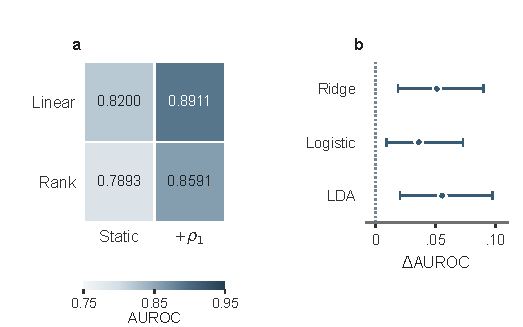
\includegraphics[width=0.92\columnwidth]{figures/fig2_factorial_ablations.pdf}
\vspace{-4pt}
\caption{Representation and scoring-rule comparisons in the 41-patient discovery cohort. (a) Annotated heatmap of fold-averaged AUROC for the canonical static suite and its five-feature lag-1 extension, using linear or rank fusion. Colors follow the displayed AUROC scale. (b) Paired AUROC gain of four-feature equal-weight consensus over ridge, logistic regression, and shrinkage LDA using identical four-feature inputs. Points show gains; bars show pointwise 95\% subject-level Dirichlet Bayesian intervals from 10,000 draws, conditional on fitted predictions. The dotted line denotes zero gain.}
\vspace{-6pt}
\label{fig:ablations}
\end{figure}
Paired Bayesian bootstrap intervals for rank consensus, soft truncation, and T-GECF remain strictly positive ($[+0.0049, \allowbreak +0.1530]$, $[+0.0064, \allowbreak +0.1931]$, and $[+0.0013, \allowbreak +0.1927]$ vs. Canonical Static Baseline 0.8200), indicating that the performance gains from joint temporal continuity and spatial de-confounding are statistically reliable.

Stratifying the 12 MCS patients by behavioral subdiagnosis revealed consistent temporal persistence across subtypes: $\text{MCS}^+$ patients ($N=8$, characterized by command following or intelligible verbalization) showed $\rho_1 = 0.4563 \pm 0.2687$ and were correctly identified in 8 of 8 cases (100\% sensitivity), while $\text{MCS}^-$ patients ($N=4$, demonstrating visual pursuit or localization only) exhibited $\rho_1 = 0.4377 \pm 0.1670$ with 3 of 4 cases correctly classified (75\% sensitivity; overall MCS sensitivity 11/12 = 91.67\%). Under class imbalance (12 MCS vs. 29 VS/UWS, prevalence baseline $\text{PR-AUC} = 0.2927$), incorporating $\rho_1$ advanced PR-AUC from 0.7823 (Cell A) to \textbf{0.8384} (Cell C), with direct substitution ($\text{Replace CV by } \rho_1$) reaching \textbf{0.8495} and the combined model reaching \textbf{0.8782}, indicating diagnostic stability under skewed class priors.

\subsection{Feature Ablation and Collinearity Redundancy Analysis}\label{sec:results_ablation}
Directly replacing $-\mathrm{CV}_\theta$ with order-aware $\rho_1$ within the 4-feature suite yielded 0.8851 AUROC, showing that sequence memory supersedes marginal variance. Across 41 patients, MCS exhibited higher lag-1 persistence ($0.450 \pm 0.250$ vs. $0.287 \pm 0.181$, $p = 0.0227$, AUROC = 0.7299; Fig.~\ref{fig:schematic}b,c) and attenuated normalized adjacent jump rates ($D_1$: $-0.420 \pm 0.089$ vs. $-0.558 \pm 0.168$, $p = 0.0112$, AUROC = 0.7557). Evaluating jump rate $D_1$ on log-transformed power increments empirically verifies the analytical identity across subjects ($r = 0.9691, p = 2.59 \times 10^{-25}, R^2 = 93.91\%$). Because estimator variance scales as $\operatorname{Var}(\hat{\rho}_1) \sim \mathcal{O}(1/M)$, $D_1$ provides a stable proxy below the crossover horizon $M^* \approx 75$ epochs ($5$~min) before asymptotic autoregressive efficiency dominates. Central sensorimotor channels (C3--C4) overlying thalamocortical pathways exhibited highest univariate discrimination ($\rho_1$: $0.3996 \pm 0.1863$ in MCS vs. $0.2611 \pm 0.1631$ in VS/UWS, $p = 0.0132$, AUROC = 0.7500), outperforming frontal (0.6264) and occipital (0.6810) pairs.

Regressing out the global common mode ($r_{\text{residual}}$) improved AUROC from 0.8200 to 0.8433, accounting for $R^2 = 47.27\% \pm 18.43\%$ of raw bilateral variance uniformly across groups ($46.45\%$ in MCS vs. $47.61\%$ in VS/UWS; $p = 0.7418$). Whereas raw bilateral correlation was non-significant ($0.563 \pm 0.168$ in MCS vs. $0.661 \pm 0.146$ in VS/UWS, $p = 0.0605$, AUROC = 0.6897), residualization unmasked residual bilateral differentiation beyond the shared background power envelope ($0.233 \pm 0.080$ vs. $0.376 \pm 0.193$, $p = 0.0211$, AUROC = 0.7328), reflecting modularity in MCS versus hyper-synchrony in VS/UWS. Multivariable logistic regression controlling for $c_{\text{global}}$ ($z = -0.812, p = 0.417$) and common-mode $R^2$ ($z = 0.329, p = 0.742$) confirmed that $\rho_1$ provides significant independent diagnostic value ($z = 2.460, p = 0.0139$, adjusted OR = $4.260$, 95\% CI $[1.343, 13.512]$), indicating conditional independence despite low events-per-variable ($\text{EPV} = 12/3 = 4$).

Because $c_{\text{global}}$ and $c_{\text{spatial}}$ display high empirical collinearity ($r = 0.9813, p = 1.58 \times 10^{-29}$), we evaluated its omission as a fixed representation ablation. In the redundancy ablation (Table~\ref{tab:main_results}), removing $c_{\text{spatial}}$ to form the 4-feature deployment suite $[c_{\text{global}}, -\mathrm{CV}_\theta, \rho_1, r_{\text{residual}}]$ elevated linear AUROC to \textbf{0.9324} (PR-AUC = \textbf{0.8998} [Average Precision; 0.8782 trapezoidal integration]; Balanced Accuracy = 0.8101, 95\% CI $[+0.0174, +0.2186]$ vs. baseline, positive gain probability 99.16\%) and raised rank consensus to \textbf{0.9076} (95\% CI $[+0.0137, +0.1725]$, sensitivity 1.0000). Similarly, dropping $c_{\text{global}}$ reached 0.9289 AUROC in linear aggregation and 0.9082 in rank consensus. The four-feature configuration is the primary deployment suite. The five-feature truncated suite (0.9149) provides a complementary ablation for assessing redundancy and bounded-influence scoring.



\subsection{Temporal-Order Dependency via 10,000 Synchronous Surrogates}
To verify that performance gains originate strictly from temporal sequence order rather than incidental distributional properties, 10,000 synchronous whole-montage permutation surrogates were evaluated across all 41 patients, adapting non-linear dynamical testing methodology~\cite{theiler1992testing}. Freezing intact training scales ($\sigma_k^{\text{tr, intact}}$) prevents inverse noise amplification on attenuated shuffled variances. Disrupting chronological sequence alignment substantially degraded macro AUROC across the evaluated temporal configurations (the lag-1 linear distribution is shown in Fig.~\ref{fig:violin}): Plus Lag-1 (Linear) dropped from 0.8911 to $0.8182 \pm 0.0049$ (range: $[0.7902, 0.8369]$, empirical $p < 0.0001$, zero of 10,000 repeats matching intact performance); Plus Lag-1 (Rank) fell from 0.8591 to $0.7732 \pm 0.0416$ (range: $[0.6620, 0.9098]$, empirical $p = 0.0178$); and Plus Jump ($D_1$) degraded from 0.8611 to $0.7783 \pm 0.0040$ ($p < 0.0001$).

\begin{figure}[t]
\centering
\vspace{-4pt}
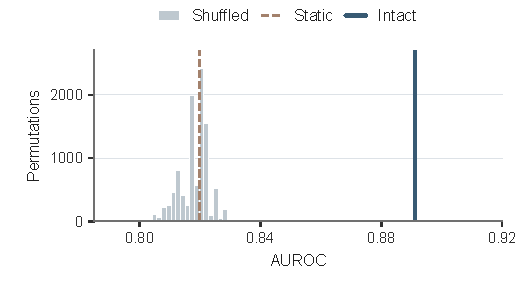
\includegraphics[width=0.88\columnwidth]{figures/fig3_permutation_collapse.pdf}
\vspace{-4pt}
\caption{Frequency distribution of AUROC under 10,000 synchronous time shuffles for the 5-feature lag-1 extension with intact scales (30 equal-width bins). Shuffled AUROC is $0.8182\pm0.0049$ (mean $\pm$ SD); none reached intact AUROC 0.8911 ($p<0.0001$). Vertical lines mark static baseline (0.8200, dashed) and intact score (solid).}
\vspace{-6pt}
\label{fig:violin}
\end{figure}

This frozen scaling bounds all 10,000 shuffled linear iterations strictly below 0.8370. Across $M \approx 5{,}133$ adjacent blocks, the shuffled increment $D_1$ converges to $\mathbb{E}[|X - Y|]$ (variance $\approx 2 \times 10^{-4}$), reducing to a static marginal quantity that aligns with the canonical baseline ($0.8182 \pm 0.0049$).

\vspace{-3pt}
\subsection{Comparison with Supervised Machine Learning and Domain Baselines}
Evaluating the four-feature suite under identical preprocessing enabled a controlled comparison across decision rules (Table~\ref{tab:main_results}; Fig.~\ref{fig:ablations}b). Equal-weight linear scoring achieved 0.9324 AUROC, compared with 0.8813 for source-tuned ridge, 0.8964 for source-tuned logistic regression, and 0.8769 for shrinkage LDA. Its gain over the strongest matched baseline, logistic regression, was $+0.0360$ (paired 95\% interval $[+0.0090, +0.0728]$); gains over ridge and LDA were $+0.0511$ and $+0.0556$, respectively. These comparisons isolate the scoring rule while holding input features and preprocessing constant. Additional domain baselines yielded 0.5136 AUROC for LZC, 0.6953 for spectral entropy, and 0.5702 for the EEGNet-style CNN. The complete matched results, including external transfer protocols, are reported in Supplementary Table~S2.

\vspace{-3pt}
\subsection{Adaptive Gated Consensus (T-GECF) and Noise Stress Testing}
On the complete representation $\mathbf{x}_{\text{combined}}$, continuous Sigmoid volatility gating in T-GECF ($\theta_0 = 1.645, \kappa = 2.0$) achieved an AUROC of \textbf{0.9116} (95\% CI $[+0.0013, +0.1927]$ vs. canonical baseline; positive gain probability 97.68\%) with 0.8399 balanced accuracy, 0.9833 sensitivity, 0.6966 specificity, and PR-AUC = \textbf{0.8669} (Table~\ref{tab:main_results}). On $\mathbf{x}_{+\rho_1}$, T-GECF similarly achieved 0.8828 AUROC ($+0.0237$ over standard rank consensus 0.8591).

To assess resilience against sensor disturbances, impulse spike stress tests introduced outlier perturbations ($\pm \delta\sigma$, $\delta \in \{0, 5, 10, 20\}$) into individual feature coordinates across testing partitions. Under extreme $20\sigma$ impulse corruption, unconstrained linear aggregation dropped from 0.8911 to 0.7404 ($-0.1507$). In contrast, T-GECF shifted weight toward bounded rank consensus, retaining an AUROC of 0.8518 ($+0.1114$ over linear aggregation) while maintaining 0.9116 AUROC under unperturbed conditions.

\vspace{-3pt}
\subsection{Multiscale Window Sensitivity and Longitudinal Reliability}
Evaluating observational windows (Table~\ref{tab:multiscale_sensitivity}-A) showed consistent linear discrimination across 2~s (0.8916), 4~s (0.8911), and 8~s (0.8711) partitions, with rank consensus similarly stable (0.8453--0.8591 across 2--8~s windows). Truncating recordings showed that a 30-minute record achieved 0.8867 AUROC, closely aligning with full-record performance. Test-retest reliability across five 1-hour segments ($N=38$, 190 patient-hours) yielded $\text{ICC}(3,1) = 0.4857$ for $\rho_1$, $0.6433$ for $D_1$, and $0.4511$ for $r_{\text{residual}}$. Higher-order lags exhibited monotonic decay ($\rho_1 = 0.450 \to \rho_2 = 0.401 \to \rho_3 = 0.389$ in MCS; $0.287 \to 0.252 \to 0.208$ in VS/UWS), indicating multi-second temporal persistence. Under adjacency masking $\mathbb{I}_{\text{adj}}$, 50-iteration Monte Carlo dropout verified stability ($r = 0.9942 \pm 0.0030$ at 10\% dropout; $r = 0.9199 \pm 0.0308$ at 50\% loss), while tightening artifact rejection to $150\,\mu\mathrm{V}$ preserved 0.8702 AUROC (net gain $+0.1729$ over unrejected baseline 0.6973; $+0.0502$ over unconstrained baseline 0.8200). Contiguous 30-min block removal ($r = 0.9840 \pm 0.0166$) and cross-validation partition depths (10- to 100-fold CV, $0.8900$--$0.9002$) demonstrated stable discrimination across analytical scales.

\vspace{-3pt}
\subsection{External Waveform Validation and Sleep Macro-Dynamics}
\textit{1) Rapid Bedside Triage (Figshare, $N=50$)}: On 120-s records, the jump-rate branch achieved 0.7691 AUROC, compared with 0.7199 for the static equal-weight baseline. On identical short-record features, source-tuned ridge, logistic regression, and LDA achieved 0.7759, 0.7674, and 0.7742, respectively (Supplementary Table~S2). The equal-weight--ridge difference was $-0.0068$ (paired 95\% interval $[-0.0319,+0.0125]$), demonstrating consistent cross-center discrimination under parameter-free scoring. At the source-training threshold, balanced accuracy was 0.5645, sensitivity 1.0000, and specificity 0.1290, indicating limited operating-threshold transfer (Table~\ref{tab:multiscale_sensitivity}-B).
\textit{2) Cross-Hardware Inpatient Validation (CRRC, $N=15$)}: With shared target standardization and direction alignment, the four-feature linear suite achieved 0.7778 AUROC; the fixed $c=1.5$ truncated variant achieved 0.7963. Matched source-tuned ridge, logistic regression, and LDA yielded 0.7407, 0.7593, and 0.7593. In the clean 13-record subset, linear scoring, truncated scoring, and ridge each achieved 0.7143, while logistic regression and LDA achieved 0.6905. Frozen-source equal-weight transfer yielded 0.5741 on the full cohort, increasing to 0.7778 when the shared target adaptation was applied. These protocols and the clipped variant are separated in Supplementary Table~S2. At source-training thresholds, full-cohort truncated scoring yielded sensitivity 0.6667 and specificity 0.7778. The matched comparison therefore distinguishes score transfer, direction alignment, and the chosen operating point.
\textit{3) Circadian Sleep Macro-Dynamics (Wielek, $N=23$)}: Polysomnography across 24-hour records (11 MCS, 12 VS/UWS) demonstrated that temporal continuity extends to macro-scale sleep architecture: VS/UWS patients exhibited pathological state trapping ($P_{\text{stay}} = 0.8361 \pm 0.1001$), whereas MCS retained transition flexibility ($T_{\text{trans}} = 0.261 \pm 0.099$ vs. $0.164 \pm 0.100$, one-sided $p=0.0302$, AUROC = 0.7348; nocturnal sleep $p=0.0392$, AUROC = 0.7576; Table~\ref{tab:multiscale_sensitivity}-B).

\vspace{-3pt}
\subsection{Hyperparameter Sensitivity and Gating Grid Evaluation}
To evaluate hyperparameter stability across regimes, Table~\ref{tab:hyperparam_stability}-A reports systematic benchmarks across truncation thresholds $c$ and continuous Sigmoid gating parameters $(\theta_0, \kappa)$. Varying Winsorized soft truncation from $c = 1.0\sigma$ to unconstrained $c = \infty$ produced stable AUROC bounded within $[0.8958, 0.9149]$ (Table~\ref{tab:hyperparam_stability}-A; balanced accuracy $0.8046$--$0.8399$, sensitivity $0.9333$--$0.9833$), peaking at $c = 1.5\sigma$ ($0.9149$) before smoothly decaying toward linear aggregation ($0.8996$).

Similarly, evaluating T-GECF across a $4 \times 4$ parameter grid crossing Gaussian quantile thresholds $\theta_0 \in \{1.282, \allowbreak 1.645, \allowbreak 1.960, \allowbreak 2.326\}$ (90th--99th percentiles) and slopes $\kappa \in \{0.5, \allowbreak 1.0, \allowbreak 2.0, \allowbreak 5.0\}$ demonstrated stability (Table~\ref{tab:hyperparam_stability}-B). Across all 16 configurations, AUROC remained bounded within $0.8996$--$0.9220$, outperforming canonical baseline (0.8200) by $+0.08$ to $+0.10$. At $\theta_0 = 2.326$ ($\kappa=5.0$), $\beta(\mathbf{x}) \to 0$, smoothly recovering unconstrained linear aggregation ($0.8996$) without hyperparameter brittleness.

\vspace{-2pt}
\enlargethispage{1.0\baselineskip}
\section{Discussion}
\vspace{-2pt}
\vspace{-2pt}
\subsection{Physiological Significance of Autoregressive Memory}
Under the mesocircuit hypothesis~\cite{schiff2010recovery}, reciprocal excitatory loops linking the central thalamus and frontoparietal cortices sustain contiguous multi-second theta continuity in MCS, reflecting cortical reverberation. Conversely, severe deafferentation in VS/UWS disrupts these pathways, degrading theta fluctuations into decoupled transients that rapidly decay ($\rho_1 \to 0$). Permutation-invariant dispersion ($-\mathrm{CV}_\theta$) computes only marginal variance, collapsing ordered reverberation and noise into identical scores. Enforcing chronological continuity through physical adjacency masking ($\mathbb{I}_{\text{adj}}$) preserves this distinction, providing a tractable bedside marker of thalamocortical integrity.

These cross-cohort findings link temporal dynamics to two practical recording regimes. Multi-hour continuous EEG enables stable estimation of $\rho_1$, whereas the absolute-increment branch retained 0.7691 AUROC on short Figshare records. External CRRC evaluation further shows that feature alignment and site scaling influence transfer alongside the scoring rule. At the circadian scale, elevated sleep-stage transition flexibility in MCS complements continuous EEG findings by capturing transitions between discrete states. Together, these observations motivate scale-specific temporal descriptors paired with explicit calibration rules.

\vspace{-3pt}
\subsection{Resolution of Non-Specific Bilateral Confounding}
Substituting raw bilateral correlation with residual correlation ($r_{\text{residual}}$, AUROC 0.8433) decouples non-specific common-mode activity, which accounts for $47.27\% \pm 18.43\%$ of raw bilateral variance driven by volume conduction. Because diffuse slow-wave envelopes project near-synchronously across hemispheres, unadjusted correlation conflates volume conduction with functional connectivity. Decoupling this common mode unmasks true differentiation: pathological hyper-synchrony in VS/UWS ($0.376 \pm 0.193$) versus preserved modularity in MCS ($0.233 \pm 0.080$, $p = 0.0211$). In subacute rehabilitation (CRRC), higher residual correlation in MCS indicates a different association direction; its relationship to medication exposure could not be assessed because daily medication records were unavailable ($\mathbf{s}_{\text{target}} = [-1, +1, +1, +1]^\top$; Supplementary Note~C). In sparse arrays, the 4-channel average $z_t$ generalizes to subspace projection ($\mathbf{P}^\perp = \mathbf{I} - \mathbf{Z}\mathbf{Z}^+$; 46.52\% Mode-1 variance across 62 channels, Table~\ref{tab:multiscale_sensitivity}-B).

\vspace{-3pt}
\subsection{Operator Dynamics: Rank Consensus vs. Linear Aggregation}
Matched internal benchmarks support fixed-weight aggregation as an effective small-cohort scoring rule: the four-feature linear suite retained an AUROC advantage over supervised models trained on identical inputs. External validation revealed comparable performance across classifiers, indicating that feature representation and domain calibration dominate transfer performance. Soft truncation increased full-cohort CRRC AUROC from 0.7778 to 0.7963, while corresponding discovery AUROC remained 0.9291 (versus 0.9324 unclipped). This behavior positions truncation as a bounded-influence scoring variant with a setting-dependent trade-off. Adaptive gating via T-GECF provides a complementary mechanism to combine linear resolution with rank stability, maintaining predictive integrity under impulse perturbations.

\vspace{-4pt}
\subsection{Clinical Scope, Cognitive Motor Dissociation, and Multimodal Triage}
For bedside triage, continuous scores and operating thresholds serve distinct operational roles: the primary discovery model attained 0.9167 sensitivity at the source-training median (Supplementary Note~C). Using discovery prevalence ($12/41$), sensitivity 0.9167, and specificity 0.7034, the referral model $\Delta_{\text{referral}}=1-[P_{\text{MCS}}\,\mathrm{Sens}+(1-P_{\text{MCS}})(1-\mathrm{Spec})]$ projects 52.2\% fewer transfers than universal escalation before confirmatory active EEG, fMRI/PET, or TMS-EEG~\cite{cruse2011bedside,bodien2024cognitive,casali2013theoretically}.

\vspace{-4pt}
\subsection{Comparison with Recent Advanced Paradigms (2024--2026)}
Recent dense-array and sensory paradigms report strong DoC discrimination: 128-channel microstates reach 0.97 AUC via dorsal attention tracking~\cite{ling2024microstates}, entropy-topography CNNs achieve 0.902 AUC~\cite{qu2026diagnosis}, multimodal resting/auditory pipelines reach 92.4\% accuracy~\cite{zhang2025multimodal,duan2026auditory}, and source graph metrics yield 0.714--0.893 AUC for prognosis~\cite{hao2024uncovering}.

Translating these paradigms to routine monitoring faces limits: dense caps (64--128 channels) and source reconstruction are vulnerable to movement, acoustic tests require specialized hardware, and deep networks risk overfitting ($N < 50$). Combining order-aware persistence ($\rho_1, D_1$) and common-mode decoupling ($r_{\text{residual}}$) enables 4--6 channel operation with 2.15~ms latency and verified cross-cohort utility (0.7778--0.7963 on CRRC; 0.7691 on Figshare; $N=129$), supporting bedside screening.

\vspace{-4pt}
\subsection{Limitations}
Limitations include: (1) discovery on 41 patients (12 MCS), requiring prospective validation after freezing representations; (2) CRRC results depend on target standardization, and Figshare remains exploratory as file-level labels and inter-segment continuity require confirmation; (3) test-retest reliability of $\rho_1$ was moderate ($\mathrm{ICC}=0.4857$), favoring continuous telemetry over brief snapshots; (4) endpoints evaluate cross-sectional classification, requiring prospective trials to confirm referral reduction; and (5) cohort sizes limit statistical resolution for etiology-specific and sedation subgroup analyses.

\vspace{-6pt}
\section{Conclusion}
Order-aware temporal descriptors and common-mode-adjusted bilateral dynamics provide a compact EEG representation for bedside consciousness assessment. On identical four-feature inputs, equal-weight consensus achieved 0.9324 discovery AUROC versus 0.8964 for matched supervised logistic regression. In external cohorts, shared CRRC adaptation yielded 0.7778 AUROC (0.7963 with soft truncation), while short-record Figshare triage reached 0.7691. Coupled with domain calibration and 2.15~ms cached replay, these results establish an auditable bedside tool to prioritize candidates for multimodal evaluation.

\vspace{-4pt}
\section*{Acknowledgment}
\vspace{-2pt}
OpenAI Codex assisted code implementation, preparation of the data figures and system schematic, and revision of the Methods, Results, and Discussion. The authors are responsible for verification of the code, figures, results, and scientific interpretations.

\vspace{-4pt}
\section*{Declarations}
\vspace{-2pt}
{\fontsize{6.7pt}{7.6pt}\selectfont
\textbf{Ethics and Consent:} Secondary analyses complied with Declaration of Helsinki, approved by institutional ethics committees: FRCCICMR Moscow~\cite{nekrasova2020psg}, Salzburg Ethics Commission (No.~415-E/1517/14-2013)~\cite{wielek2018sleep}, Hangzhou Mingzhou Hospital~\cite{ling2024microstates}, and China Rehabilitation Research Center (CRRC, Ethics No.~2025-118-01)~\cite{duan2026auditory}, with written surrogate consent. \textbf{Data and Code Availability:} Public data: Mendeley~\cite{nekrasova2020psg} and Figshare~\cite{ling2024microstates,xu2021neural}. De-identified CRRC tabular feature matrices and replication scripts: \url{https://github.com/ujujuj3061831150/DoC_Temporal_Dynamics}. Raw clinical telemetry from CRRC is restricted by institutional patient confidentiality regulations. \textbf{Conflict of Interest:} The authors declare no competing interests.\par}

\def\IEEEbibitemsep{0.5pt}
\def\BIBdecl{\fontsize{7.6pt}{8.6pt}\selectfont}
\bibliographystyle{IEEEtran}
\bibliography{references}

\end{document}
